\documentclass{beamer}
\usepackage[latin1]{inputenc}
\usetheme{CambridgeUS}
%\usetheme{Warsaw}
\usefonttheme[onlymath]{serif}
\title[MAB-based CMA-ES]{Multi-armed Bandit Based Covariance Matrix Adaptation
Evolution Strategy}
\author[Chuan-Che Yen]{Chuan-Che Yen \\Advisor: Dr. Tian-Li Yu}
\institute{TEILab}
\date{Nov 27, 2014}


%\setbeamercovered{transparent}
\usepackage{amsfonts}

%rendering images
\usepackage{graphicx}
\graphicspath{{./img/}}

%for algorithm
\usepackage[linesnumbered]{algorithm2e}

\AtBeginSection[]{
  \begin{frame}<beamer>
    \frametitle{Outline}
    \tableofcontents[
      currentsubsection,
      sectionstyle=show/shaded,
      subsectionstyle=show/show/hide,
    ]
  \end{frame}
}

\begin{document}

\begin{frame}
  \titlepage
\end{frame}
\begin{frame}
  \frametitle{Outline}
  \tableofcontents[
    currentsubsection,
    sectionstyle=show/show,
    subsectionstyle=show/hide,
  ]
\end{frame}



%

\section{Real-valued Function Optimization}

\begin{frame}{Real-valued Function Optimization}
  \begin{itemize}
    \item{Real-valued function}
      \begin{itemize}
        \item $f \colon \mathcal{S} \subset \mathbb{R}^n \to
          \mathbb{R},x \mapsto f(x)$
        \item $\mathcal{S} \colon $ search space
        \item Elements of $\mathcal{S} \colon $ candidates or solutions
      \end{itemize}
    \item{Optimization}
      \begin{itemize}
        \item $\mathop{\arg\min}\limits_{x} f(x)$, where $x$ are within given bounds.
        \item Maximizing $f$ is equivalent to minimizing $-f$.
      \end{itemize}
    \item Example
      \begin{itemize}
        \item $\mathop{\arg\min}\limits_x 2x^3-3x^2-36x-14$.
        \item Design of aircraft wings.
      \end{itemize}
  \end{itemize}
\end{frame}

\begin{frame}{Black-box Optimization}

  \begin{itemize}
    \item Without interior information.
    \item Unavailable to optimize using mathematical methods. 
    \item The only information is the interaction between input and
      output.  
  \end{itemize}
  \begin{figure}[b]
    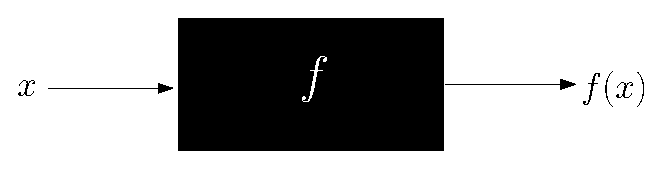
\includegraphics[scale=0.5]{BlackBox.eps}
    \caption{Black-box function}  
  \end{figure}

\end{frame}

\begin{frame}{Difficulties}
  \begin{columns}
    \begin{column}{0.6\textwidth}
      \begin{itemize}[<+->]
        \item Non-convex
          \begin{itemize}
            \item Multi-modal problems
          \end{itemize}
        \item <.(-2)-> Ruggedness
          \begin{itemize}  
            \item Perturbated by noise. 
            \item Non-smooth.
          \end{itemize}
        \item <.(-3)-> Dimensionality and non-separable
        \item <.(-3)-> Ill-conditioned
          \begin{itemize}
            \item Unable to extract gradient information
          \end{itemize}
      \end{itemize}
    \end{column}
    \begin{column}{0.4\textwidth}
      \onslide<2->{
        \begin{figure}[l]
          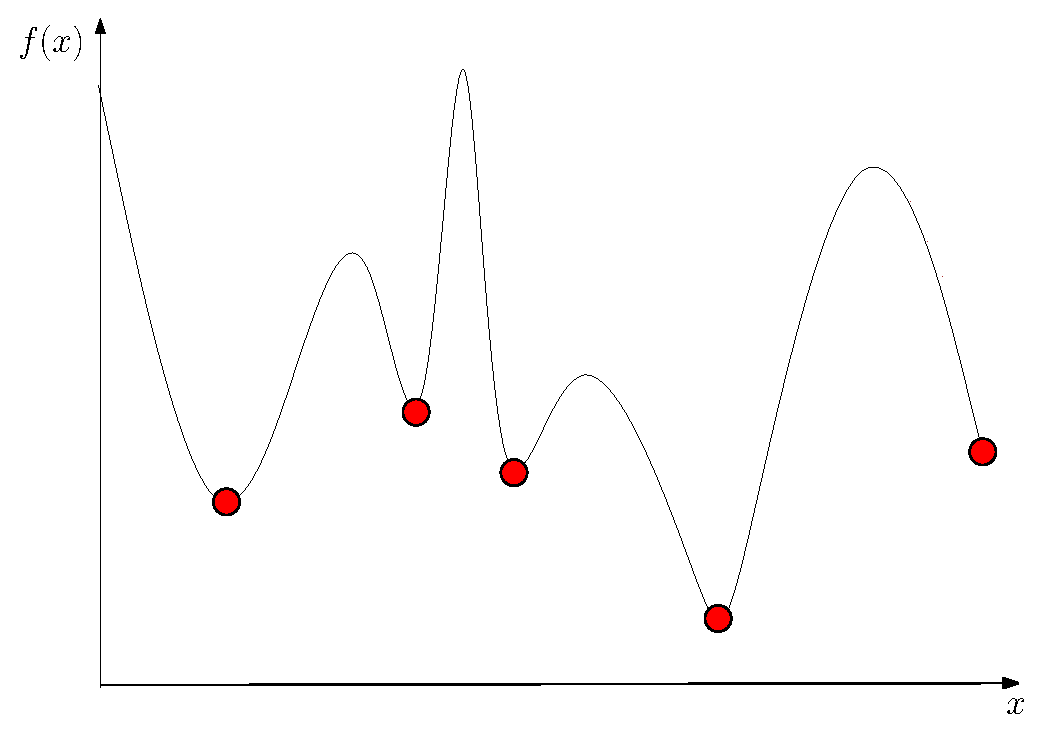
\includegraphics[width = 0.6\columnwidth]{Non-Convex.eps}
          \caption{Non-convex function}
        \end{figure}
      }
      \onslide<4->{
        \begin{figure}[H]
          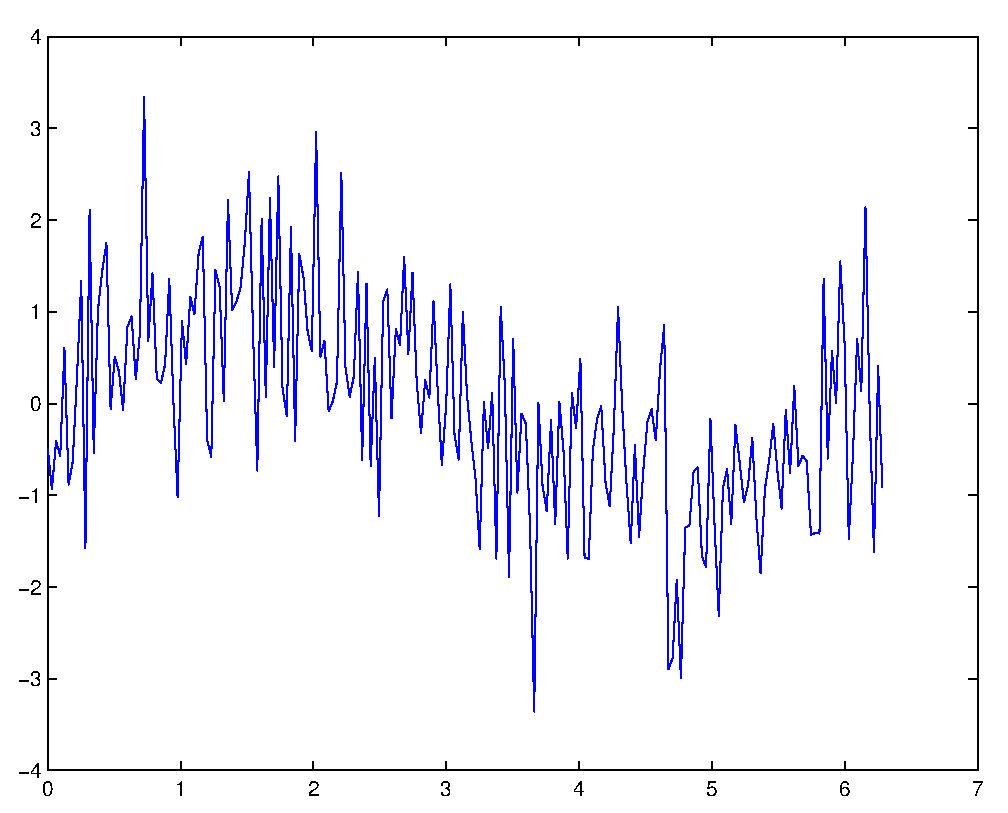
\includegraphics[width = 0.6\columnwidth]{Rugged.eps}
          \caption{$sin(x)$ with noise}
        \end{figure}
      }
    \end{column}
  \end{columns}
\end{frame}

%\section{Related Approaches}
\begin{frame}{Related Approaches}
  \begin{itemize}
    \item Optimization
      \begin{itemize}
        \item Deterministic
        \item Stochastic
      \end{itemize}
      \vspace*{14pt}
    \item Properties
      \begin{itemize}
        \item Stability
        \item Robustness
      \end{itemize}
      \vspace*{14pt}
    \item Utilizing global information
      \begin{itemize}
        \item Estimation of Distribution Algorithm (EDA)
        \item Model building
      \end{itemize}
  \end{itemize}
\end{frame}

\subsection{Real-coded Extended Compact Genetic Algorithm}


\begin{frame}{Discretization} 
  \begin{itemize} 
    \item Continuous domain $\rightarrow$ Discrete domain 
    \item Finding good solutions $\rightarrow$ Finding promising
      regions
    \item 2 traditional discretization methods
      \begin{itemize}
        \item Fixed-Height Histogram (FHH)
        \item Fixed-Width Histogram (FWH)
      \end{itemize}
      \vspace*{2pt}
  \end{itemize}
  \begin{minipage}{.45\textwidth}
    \begin{figure}
      \centering
      \includegraphics[bb = 144 82 686 502, clip, width =0.9\textwidth]{FHH.eps}
      \caption{FHH}
    \end{figure}
  \end{minipage}
  \begin{minipage}{.45\textwidth}
    \begin{figure}
      \centering
      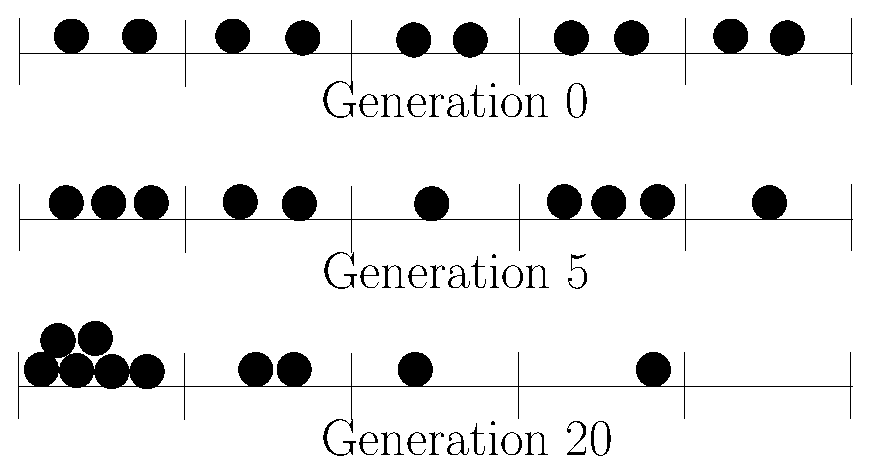
\includegraphics[bb = 144 82 686 502, clip, width =0.9\textwidth]{FWH.eps}
      \caption{FWH}
    \end{figure}
  \end{minipage}

\end{frame}

\begin{frame}{Split on Demand}
  \begin{itemize}
    \item Solutions in each bin should not exceed $\gamma N$.
      \begin{itemize}
        \item $N$ is the population size.
        \item $\gamma$ defines the rate of one region.
      \end{itemize}
    \item $\gamma$ decays with a factor $\epsilon$.
  \end{itemize}
  \begin{figure}[h]
    \includegraphics[bb = 100 86 635 502, clip, scale = 0.3]{SoD.eps}
    \caption{SoD}
  \end{figure}
\end{frame}

%\begin{frame}{EDA}
%  \begin{columns}
%    \begin{column}{.5\textwidth}
%      \begin{itemize}
%        \item Sometimes known as Probabilistic Model Building GA (PMBGA).
%          \begin{itemize}
%            \item Building model explicitly.
%            \item Linkage between decision variables are provided.
%          \end{itemize}
%          \vspace*{14pt}
%          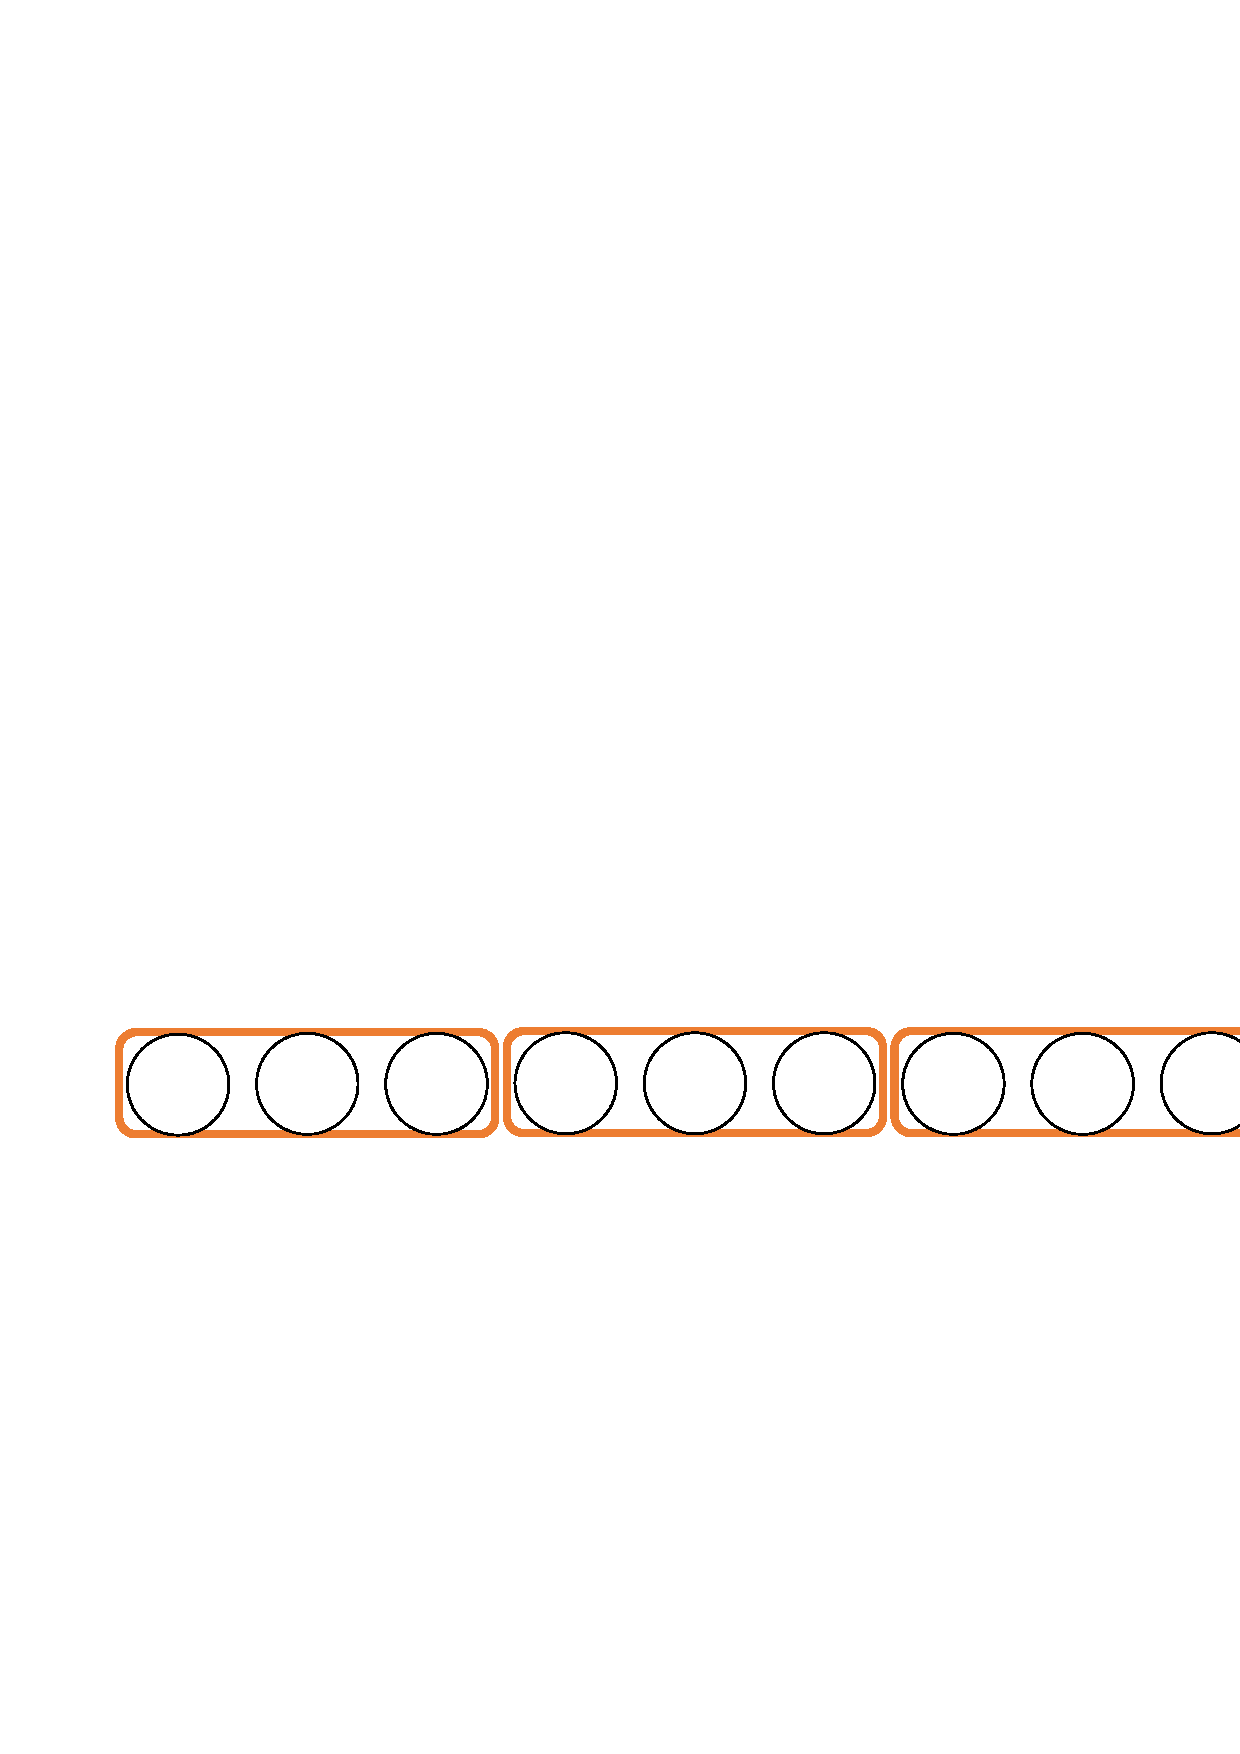
\includegraphics[bb= 46 359 625 282, clip, width = 0.8\textwidth]{linkage}
%      %  \item  Extended Compact Genetic Algorithm (ECGA).
%      %    \begin{itemize}
%      %      \item Model is built according to population distribution.
%      %      \item Applying greedy search to refine model iteratively.
%      %    \end{itemize}
%      \end{itemize}
%    \end{column}
%    \begin{column}{.5\textwidth}
%      \begin{figure}[htp]
%        \centering
%        \includegraphics[width = 0.8\textwidth]{EDA.eps}
%      \end{figure}
%    \end{column}
%  \end{columns}
%\end{frame}

\begin{frame}{Extended Compact Genetic Algorithm}
  \begin{figure}
    \centering
  \includegraphics[bb = 1 125 900 450, clip, height = 0.35\textheight]{EDA2.eps}
\end{figure}
  \begin{figure}
    \centering
  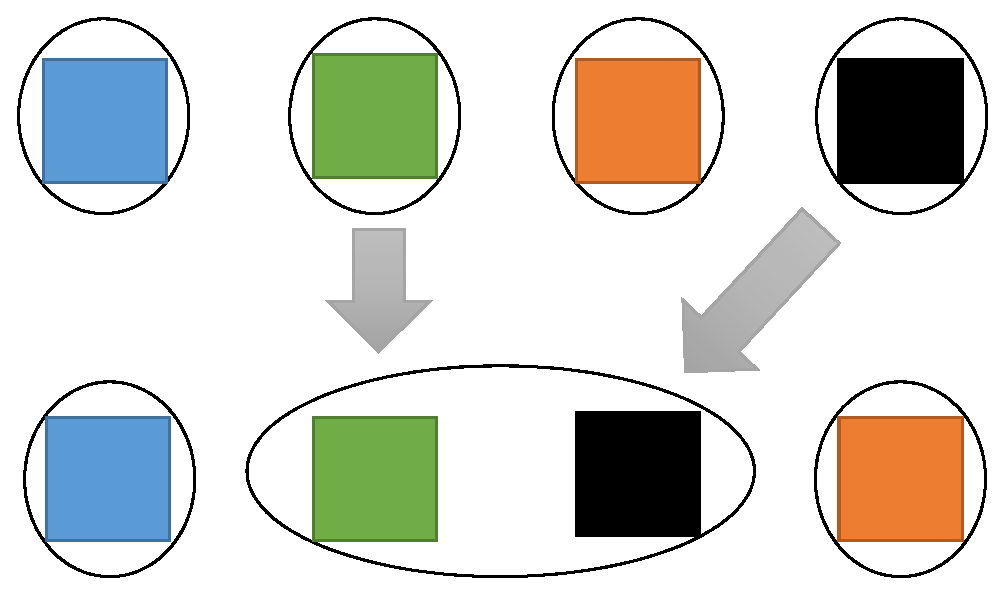
\includegraphics[bb = 32 150 552 450, clip, height = 0.15\textheight]{modelbuilding.eps}
\end{figure}
  \begin{itemize}
    \item $Pr(x_1,x_2,x_3,x_4) = Pr(x_1)Pr(x_2,x_4)Pr(x_3)$
  \end{itemize}
\end{frame}

\begin{frame}{Extended Compact Genetic Algorithm}
  \begin{figure}[t]  
    \includegraphics[bb = 50 73 777 554, clip, width=.8\textwidth]{ECGA.eps}
  \end{figure}
\end{frame}

\begin{frame}{Real-coded ECGA with SoD}
  \begin{figure}[t]  
    \includegraphics[bb = 50 73 777 554, clip, width=.8\textwidth]{rECGA.eps}
  \end{figure}

\end{frame}

\begin{frame}
  \frametitle{rECGA}
  \begin{itemize}
    \item Discretization 
      \begin{itemize}
        \item Continuous domain $\rightarrow$ Discrete domain $\rightarrow$
          Continuous domain
        \item Any distortion?
      \end{itemize}
  \end{itemize}
  \begin{figure}[htpb]
    \includegraphics[bb= 92 220 755 397, clip, width=0.5\textwidth]{Discretization.eps}
  \end{figure}
  \begin{itemize}
    \item Sampling
      \begin{itemize}
        \item Cliff between each bin is sometimes steep.
      \end{itemize}
      \begin{figure}[hpb]
        \includegraphics[bb = 67 21 774 546,clip, width = 0.3\textwidth]{Sampling.eps}
      \end{figure}
  \end{itemize}

\end{frame}


\begin{frame}{rECGA}
  \begin{itemize}
    \item rECGA tackles the difficulty of \alert{dimensionality}.
      \vspace*{14pt}
    \item Struggles in exploration, sampling.
      \vspace*{14pt}
    \item Why not solve continuous problem right in continuous domain?
  \end{itemize}
\end{frame}

\subsection{Covariance Matrix Adaptation Evolution Strategy}


\begin{frame}{Evolution Strategy (ES)}
  \begin{itemize}
    \item A search template for black-box optimization.
      \begin{itemize}
        \item Encoded in continuous domain.
      \end{itemize}
      \vspace*{14pt}
    \item New search points are generated based on current population.
      \vspace*{14pt}
    \item $x_i^{t+1} = m^t + \sigma N_i(0,C)$.
      \begin{itemize}
        \item $x_i^{t+1}$: $i$-th generated solution at generation $t+1$.
        \item $m^t$: weighted mean of population at generation $t$.
        \item $\sigma$: step size.
        \item $C$: Estimated distribution.
      \end{itemize}
  \end{itemize}
\end{frame}

\begin{frame}{Covariance Matrix Adaptation Evolution Strategy (CMA-ES)}
  \begin{itemize}
    \item A famous branch of ES
      \vspace*{14pt}
    \item Importance of $\sigma$ and $C$.
      \begin{itemize}
        \item Larger step size reinforces exploration while smaller
          reinforces exploitation.
          \begin{itemize}
            \item Choosing an fixed, appropriate number?
          \end{itemize}
        \item Covariance matrix determines the shape of estimated
          distribution.
          \begin{itemize}
            \item Determining the length of each axis.
            \item Representing the dependency among decision variables.
          \end{itemize}
      \end{itemize}
      \vspace*{14pt}
    \item CMA-ES features in the adoption of historical information.
      \begin{itemize}
        \item $\sigma$ and $C$ are adjusted accordingly.
      \end{itemize}
  \end{itemize}
\end{frame}

\begin{frame}{CMA-ES}
  \begin{figure}[t]
    \includegraphics[bb= 79 64 664 552, clip, width = 0.75\textwidth]{CMAES.eps}
  \end{figure}
\end{frame}

\begin{frame}{CMA-ES}
  \begin{itemize}
    \item An outstanding local optimizer
    \item Tackles \alert{non-separable} by maintaining a
      covariance matrix
    \item Usually encounters premature convergence
  \end{itemize}
  \begin{figure}[htpb]
    \centering
    \vfill\includegraphics[scale = 0.3]{LocalOptima.eps}
  \end{figure}
\end{frame}
%        \item Outer layer for exploration
%      \end{itemize}
%  \end{itemize}

%  \begin{columns}
%    \begin{column}{.33\textwidth}
%      \begin{figure}
%        \centering
%        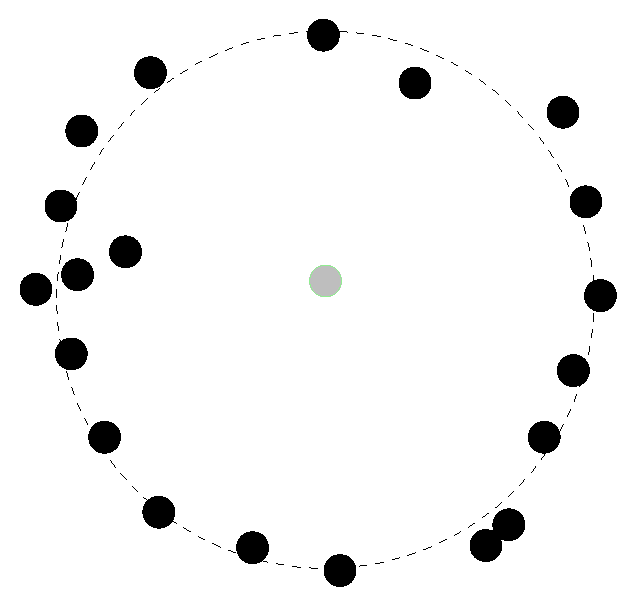
\includegraphics[width=.9\textwidth]{ES_0.eps}
%        \caption{$t$ = 0}
%      \end{figure}
%    \end{column}
%    \begin{column}{.33\textwidth}
%      \begin{figure}
%        \centering
%        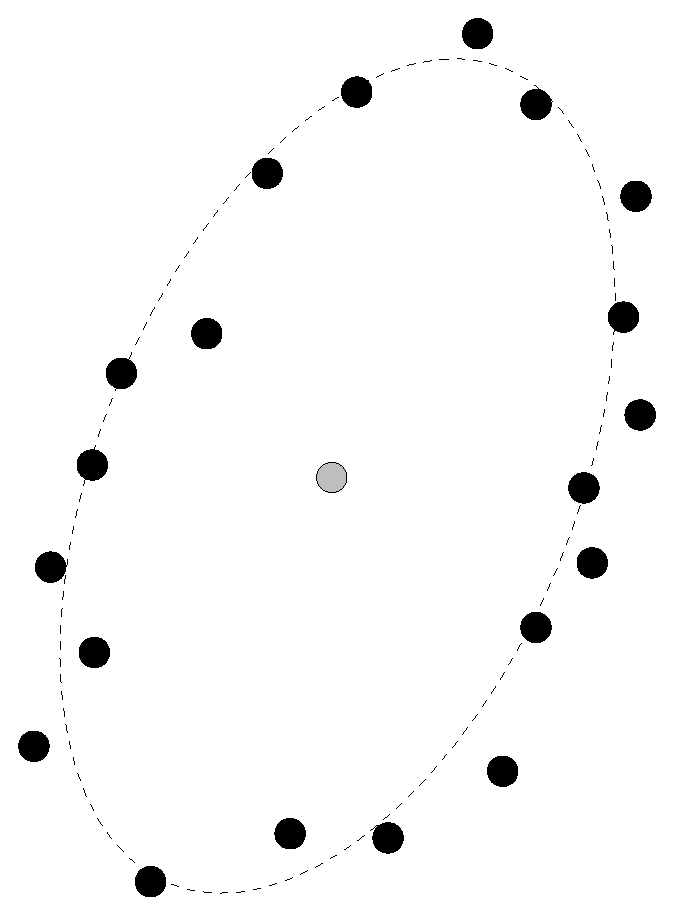
\includegraphics[width=.9\textwidth]{ES_10.eps}
%        \caption{$t$ = 10}
%      \end{figure}
%    \end{column}
%    \begin{column}{.33\textwidth}
%      \begin{figure}
%        \centering
%        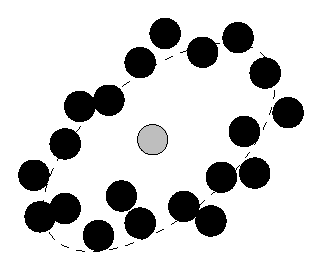
\includegraphics[width = .9\textwidth]{ES_20.eps}
%        \caption{$t$ = 20}
%      \end{figure}
%    \end{column}
%  \end{columns}


\section{Motivation}

\begin{frame}{Hypothesis}
  \begin{itemize}
    \item Both CMA-ES and rECGA suffer from \alert{ruggedness} for
      insufficient exploration.
      \vspace*{8pt}
    \item What if there is implicit information between local optima?
    \item We are interested in rugged problems with implicit tendency
  \end{itemize}
  \vspace*{10pt}
  \begin{figure}[hp]
    \centering
    \includegraphics[scale=0.25]{Problem.eps}
  \end{figure}
\end{frame}

\begin{frame}{Hypothesis}
 % \begin{itemize}
 %   \item Assume problems are with such structure
      \vspace*{10pt}
 %   \item We are aiming to fetch more promising region by evolving the
 %     tendency
 % \end{itemize}
  \setbeamercolor{block title}{use=structure,fg=white,bg=red}
  \setbeamercolor{block body}{use=structure,fg=black,bg=white!20!white}

  \begin{block}{Assumption}
   The information of the region where the global optimum resides is
   somehow hidden in the locations of local optima and can be retrieved
   by proper methods.
  \end{block}
  \begin{figure}[hp]
    \centering
    \includegraphics[bb= 40 43 658 565, clip, scale=0.25]{tendency.eps}
  \end{figure}
\end{frame}
\begin{frame}{Hypothesis}
  \begin{itemize}
    \item An enhanced exploration  
      \vspace*{10pt}
    \item Clustering based on spatial locality  
  \vspace*{10pt}
\item Performing a 2nd layer CMA-ES for evolving the tendency
  \end{itemize}
  \vspace*{10pt}
  \begin{figure}[htpb]
    \centering
    \includegraphics[scale=0.25]{hypothesis_discretization.eps}
  \end{figure}
\end{frame}

\begin{frame}{Expected benefit}
  \begin{itemize}
    \item A soft, adaptive exploration
      \begin{itemize}
        \item Iteratively exploring better regions.
        \item Generated regions are also source for better regions.
      \end{itemize}
      \vspace*{14pt}
    \item Each region can be highly exploited. 
      \begin{itemize}
        \item 1st layer CMA-ES quickly outputs local optimum.
      \end{itemize}
  \end{itemize}
\end{frame}




%\begin{frame}{Hypothesis}
%
%  \begin{itemize}
%    \item Increasing diversity by maintaining multiple groups.
%      \begin{itemize}
%        \item kind of discretization.
%        \item How to define the number of groups?
%        \item What is the criteria for individuals to form a group?
%      \end{itemize}
%      \vspace*{14pt}
%    \item There is implicit information hidden between groups.
%      \begin{itemize}
%        \item How to extract the information?
%        \item How to benefit from the information and obtain
%          better solutions?
%          \begin{itemize}
%            \item Inspired by discretization, we aim to find a more
%              promising region.
%          \end{itemize}
%      \end{itemize}
%      \vspace*{14pt}
%    \item 2-layer CMA-ES is introduced
%      \begin{itemize}
%        \item Inner layer for exploitation
%        \item Outer layer for exploration
%      \end{itemize}
%  \end{itemize}

%\end{frame}

\section{Methodology}

\begin{frame}{Flow of Proposed Template}
  \begin{columns}
    \begin{column}{0.9\textwidth}
      \begin{figure}[b]
        \vspace*{1cm}        
        \includegraphics[width = 0.6\textwidth]{Flow.eps}\hspace*{2cm}
        \caption{Flow}
      \end{figure}
    \end{column}
  \end{columns}
\end{frame}

\begin{frame}
  \frametitle{Pseudo-code of Template}

  \scalebox{0.8}{%
    \begin{algorithm}[H]
      \Begin{
        Initializing population\;
        Clustering\;
        \While{not terminate}{
          \While{any group has not been evolved for certain generation}{
            Evolving each group\;
          }
          Selecting candidates for each group\;
          Evolving the selected solutions\;
        } 
      }
      \TitleOfAlgo{Overview for the system}
    \end{algorithm}
  }
\end{frame}   

\begin{frame}{Undetermined Components}
  \begin{itemize}
    \item The method for making division
      \vspace*{14pt}
    \item The criterion of selecting representative solutions for
      each group
      \vspace*{14pt}
    \item The method for evolving the selected candidates
  \end{itemize}
\end{frame}

\begin{frame}{Making Division}
  \begin{itemize}
    \item The initial population is expected to categorized according to position.
      \begin{itemize}
        \item Roughly expresses the diversity
        \item A population in a specific region is expected driven
          toward the identical local optimum.
        \item In other words, a group can be roughly viewed as points
          near by one specific valley. 
      \end{itemize}
      \vspace*{14pt}
    \item Space locality plays an important role.
      \begin{itemize}
        \item Applying clustering
      \end{itemize}
  \end{itemize}
\end{frame}

\begin{frame}{\emph{k-means}}
  \begin{itemize}
    \item \emph{k-means} clustering is a basic method for vector quantization.
      \begin{itemize}
        \item Partitioning $n$ solutions into $k$ mutual independent
          clusters.
        \item Serving as a prototype
      \end{itemize}
      \vspace*{14pt}
    \item Number of clusters
      \begin{itemize}
        \item As known as number of groups.
        \item Without $k$, finding optimal is said to be NP-hard.  
        \item To define a proper $k$ is difficult.
      \end{itemize}
      \vspace*{14pt}
    \item  Heuristic algorithms for approximation.
      \begin{itemize}
        \item Forgy method for initialization
        \item iteratively refinements until convergence
      \end{itemize}

  \end{itemize}
\end{frame}

\begin{frame}{Algorithm of Approximation to k-means}

  \scalebox{0.8}{%  
    \begin{algorithm}[H]
      \label{algo:kmeans}
      \KwIn{$k$, $d$, $\{o_1, o_2,\ldots, o_n\}$ as observations} 
      \KwOut{$\mathcal{S}$} 
      Initial: $m_1, m_2,\ldots, m_k$ are
      random selected from observations as initial centers 
      \tcp*{Forgy method}
      \While{At least one of the observations moves to other group} 
      {\For{j = 1 to k} 
      {$S_j = \emptyset$  \;} 
      \For{i = 1 to n} {assign $o_i$ to $S_j$ if $o_i$ is
      closest to $m_j$ among the $k$ centers\;} 
      \For{j = 1 to k} {$m_j$ is updated by the arithmetic mean of all vectors $\in S_j$\;}
    }
    \TitleOfAlgo{Clustering heuristic function}
  \end{algorithm}
}

\end{frame}

\begin{frame}{Illustration for The Algorithm}
  \begin{columns}

    \begin{column}{0.23\textwidth}
      \begin{figure}[h]
        \centering
        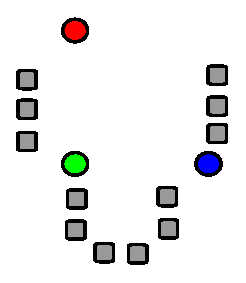
\includegraphics[scale = 0.5]{K_Means_Example_Step_1.eps}
      \end{figure}
    \end{column}

    \begin{column}{0.23\textwidth}
      \begin{figure}[h]
        \centering
        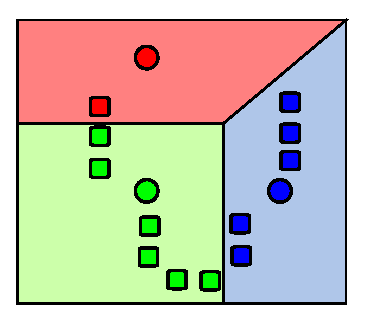
\includegraphics[scale = 0.5]{K_Means_Example_Step_2.eps}
      \end{figure}
    \end{column}

    \begin{column}{0.23\textwidth}
      \begin{figure}[h]
        \centering
        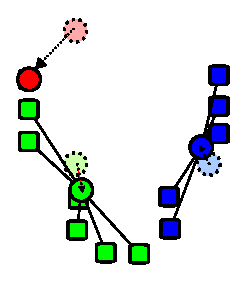
\includegraphics[scale=0.5]{K_Means_Example_Step_3.eps}
      \end{figure}
    \end{column}

    \begin{column}{0.23\textwidth}
      \begin{figure}[h]
        \centering
        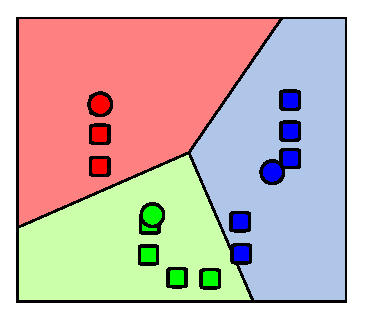
\includegraphics[scale = 0.5]{K_Means_Example_Step_4.eps}
      \end{figure}
    \end{column}
  \end{columns}
\end{frame}

\begin{frame}{Remaining Criteria}
  \begin{itemize}
    \item How to select representativeness from each group?
      \begin{itemize}
        \item Using the optimal solution found so far as the representativeness in
          each group
      \end{itemize}
      \vspace*{14pt}
    \item How to evolve selected candidates?
      \begin{itemize}
        \item Evolving them with CMA-ES
        \item The so-called `outer CMA-ES'
        \item Aims to observe if better regions can be reached
      \end{itemize}
      \vspace*{14pt}
    \item The number of solutions in a group is fixed after clustering.
      \begin{itemize}
        \item Once a better solution is generated, the worst one should
          be replaced.
      \end{itemize}
  \end{itemize}
\end{frame}

\begin{frame}{An Implementation of the Template}
  \scalebox{0.8}
  {
    \begin{algorithm}[H]{
        \KwIn{$n$,$t$}
        \KwOut{best solution ever evolved}
        Uniformly sampled population of size $n$\;
        $k = \sqrt{\frac{n}{2}}$\;
        Integrating \emph{k-means} with \emph{Frogy-method} to cluster the
        $n$ individuals into $k$ groups\;

        $C\leftarrow$ array with size $k$\;
        \For{i = 1 to k}
        {
          Optimizing group$_i$ by adopting CMA-ES for $t$ generations\;
          $C_i\leftarrow$ best solution\;
          Applying CMA-ES to evolve the population consisting of local
          optima of groups, as known as $C$, until terminated.\;
        }
      }
      \TitleOfAlgo{2-layer CMA-ES}
    \end{algorithm} 
  }
\end{frame}

\begin{frame}
  \begin{itemize}
    \item 2-layer CMA-ES addresses the diversity for the search.
      \vspace*{14pt}
    \item Next we lay emphasis on finding more promising regions.
  \end{itemize}

\end{frame}

\begin{frame}{Exploring}
  \begin{itemize}
    \item Based on current groups, we aim to figure out better
      solutions.
      \begin{itemize}
        \item According to our hypothesis, the implicit information is
          hidden between groups.
        \item What is a good way to evolve groups?
      \end{itemize}
      \vspace*{14pt}
    \item We consider the priority
      \begin{itemize}
        \item Put less concentration on groups which performs badly
        \item Lay emphasis on possible regions
        \item Without any prior knowledge, a selection strategy is
          demanded.
      \end{itemize}
      \vspace*{14pt}
    \item The ability to generate new groups adaptively 
      \begin{itemize}
        \item We assume a fixed number of groups.
        \item A replacement strategy is demanded accordingly.
      \end{itemize}
  \end{itemize}
\end{frame}

\begin{frame}{The Selection Strategy}

  \begin{itemize}
    \item The selection strategy is with the feature that
      \begin{itemize}
        \item Given a set of groups, the performance of each group is
          evaluated through trials
        \item Lays emphasis on better performance groups
        \item groups with worse performance would not be ignored
          permanently
      \end{itemize}
      \vspace*{14pt}
    \item This is just identical to the Multi-armed Bandit (MAB)
      problem.
  \end{itemize}
\end{frame}

\begin{frame}{Multi-armed Bandit Problem}
  \begin{itemize}
    \item Investigate the trade-off between exploration and exploitation
      \vspace*{14pt}
    \item Assume there are $k$ independent slot machines
      \vspace*{14pt}
    \item Each machine generates reward according to its own unknown probability
      distribution.
      \vspace*{14pt}
    \item We can only observe the playing sequence and the correlated
      reward.
      \vspace*{14pt}
    \item The goal is to maximize reward in limited play times.
  \end{itemize}
\end{frame}

\begin{frame}{Upper Confidence Bound }
  \begin{itemize}
    \item A family of solutions to MAB problems
      \vspace*{14pt}
    \item UCB1 -- the first Upper Confidence Bound (UCB) algorithm
      \vspace*{14pt}
    \item Play machine $j$ which maximizes
      \[\bar{x_j} + \sqrt{\frac{2\ln n}{n_j}}\]
      \begin{itemize}
        \item $\bar{x_j}$: the average reward of machine $j$.
        \item $n_j$: the number of times machine $j$ has been played.
        \item $n$: the played times of overall system.
      \end{itemize} 
  \end{itemize}
\end{frame}

\begin{frame}{UCB1-tuned}
  \begin{itemize}
    \item UCB1 takes no variance into consider.
      \begin{itemize}
        \item UCB1-tuned is the version which adds variance as a factor.
        \item UCB1-tuned is not proven working well but outperforms UCB1 in
          practice.
        \item In UCB1-tuned, the machine $j$ to be played is with the
          highest \[\bar{x_j} + \sqrt{\frac{\ln{n}}{n_j}
          \min(\frac{1}{4},V_j(n_j))}\], where $V_j(t) =\sigma_j^2 +
          \sqrt{\frac{2\ln n}{n_j}}$.
      \end{itemize}
      \vspace*{14pt}
    \item UCB1-tuned is adopted in our work.
  \end{itemize}

\end{frame}

\begin{frame}{The Replacement Strategy}
  \begin{itemize}
    \item By generating a new point and sampling around the new point,
      we claim to form a better group, and the worst one should be
      replaced.
      \vspace*{14pt}
    \item There are 2 judgement to distinguish if there is any group to
      delete.
      \begin{enumerate}
        \item If a group does not sample a better solution anyway.
        \item If no group converges, check among groups if there is
          group has not been played for $t$ rounds where $t$ is a
          number larger than the number of the solutions the group
          contains.
      \end{enumerate}
  \end{itemize}
\end{frame}

\begin{frame}{Flow of MAB-based CMA-ES}
  \begin{figure}[h]
    \vspace{15mm}\includegraphics[scale=0.4]{FlowMAB.eps}\hspace{25mm}
  \end{figure}
\end{frame}

\begin{frame}{Procedure of MAB-based CMA-ES}
  \scalebox{0.7}{
    \begin{algorithm}[H] 
      \TitleOfAlgo{MAB-based CMA-ES} 
      \KwIn{$n$,$t$ as a proper generation for each pulling action}
      \KwOut{best solution ever evolved} 
      Uniformly sampled population of size $n$\; 
      $k = \sqrt{\frac{n}{2}}$\; 
      Integrating \emph{k-means} with \emph{Frogy-method} to cluster the $n$ individuals into
      $k$  groups as known as bandits\; 
      $C\leftarrow$ array with size $k$\;
      \For{i = 1 to k}            
      { pull($i$)\; $C_i\leftarrow$ best
      solution\; } 
      \While{not terminated} 
      { \For{i = 1 to k} {
        calculateUCB($i$) \tcp*[r]{calculate modified UCB1-tuned as
        illustrated above} record the index with max value in $M$\;

      } 
      pull($M$)\;      
      $C_M \leftarrow$ best solution in
    group$_M$\; update()\; }
  \end{algorithm}  }
\end{frame}

\begin{frame}
  \scalebox{0.65}{
    \begin{algorithm}[H]
      Initial $P\leftarrow $ a permutation array from $1$ to $k$\; 
      ToBeDeleted = $0$\;
      \For{i = 1 to k} 
      {
        \If{deleting criterion 1 is met in group$_{P_i}$} 
        {
          ToBeDeleted = $P_i$\; 
        }  

      }
      \If{ToBeDeleted = 0} 
      {
        \For{i = 1 to k} 
        {
          \If{deleting criterion 2 is met in group$_{P_i}$}
          {
            ToBeDeleted = $P_i$\;
          } 
        } 
      } 
      \If{ToBeDeleted = 0} 
      { 
        return\; 
      } 
      \Else
      { 
        $s\leftarrow$ ToBeDeleted\; 
        generate a new solution as a new group  denoted as $group^\star$ according to $C_1, C_2,\ldots, C_{s_{i-1}}, C_{s_{i+1}},\ldots, C_k$ \; 
        \For{i = 1 to $\|group_{s}\|-1$} 
        { pull($group^\star$) without replacing worst\; }
        replace $group_{s}$ with $group^\star$\; return\; 
      } 
      \TitleOfAlgo{update}
    \end{algorithm} 
  }
\end{frame}

\section{Experiments and Results}

\begin{frame}{Testbed}
  \begin{itemize}
    \item A set of benchmark proposed in CEC 2005 (Suganthan et al. 2005) 
      \vspace*{14pt}
    \item 25 problems are categorized into 4 kinds of problem that
      \begin{itemize}
        \item Unimodal functions (1--5)
        \item Basic multi-modal functions (6--12)
        \item Expanded functions (13--14)
        \item Hybrid composition functions (15--25)
      \end{itemize}
      \vspace*{14pt}
    \item Benchmark criteria
      \begin{itemize}
        \item $N_{f_e}$ to convergence
        \item The accuracy after $10^5$ $N_{f_e}$ 
        \item We aim to design an algorithm with the ability to adaptively
          develop more promising. Therefore we take the latter.
      \end{itemize}
  \end{itemize}
\end{frame}

\begin{frame}{Experiments Design}
  \begin{itemize}
    \item The algorithms are designed based on the assumption of
      increasing diversity and extracting implicit information.
      \vspace*{14pt}
    \item As a consequence, we demonstrate 2 comparisons to verify the
      assumption.
      \begin{enumerate}
        \item Comparing original CMA-ES and  2-layer CMA-ES
        \item Comparing 2-layer CMA-ES and MAB-based CMA-ES
      \end{enumerate}
      \vspace*{14pt}
    \item Finally, a comparison between MAB-based CMA-ES and rECGA with
      SoD is demonstrated. The motivation is to verify if our algorithm
      provides comparable results in the field of discretization.
  \end{itemize}
\end{frame}

\begin{frame}{Comparison}
  \begin{itemize}
    \item For original CMA-ES, the $\lambda$ is set to 20 and $\sigma$
      is initialized to 1.
    \item For 2-layer CMA-ES, the $\lambda$ and $\sigma$ is as above.
    \item For 2-layer CMA-ES, the initial population size is set to 450
      and inner CMA-ES executes for $1000$ generations.
  \end{itemize}
  \begin{columns}
    \footnotesize
    \begin{column}{0.4\textwidth}
      \begin{table}[h]
        \begin{tabular}{|c|c|c|}
          \hline
          & CMA-ES & 2-Layer CMA-ES \\ \hline
          U & --     & --             \\ \hline
          B & --     & 1              \\ \hline
          E & --     & 2              \\ \hline
          H & 2      & 4              \\ \hline
          Total & 2 & 7 \\\hline
        \end{tabular}
        \caption{Best accuracy comparison}
      \end{table}
    \end{column}
    \begin{column}{0.4\textwidth}
      \begin{table}[h]
        \begin{tabular}{|c|c|c|}
          \hline
          & CMA-ES & 2-Layer CMA-ES \\ \hline
          U     & 1      & --             \\ \hline
          B     & 2      & 1              \\ \hline
          E     & --     & 2              \\ \hline
          H     & 3      & 5              \\ \hline
          Total & 6      & 8              \\ \hline
        \end{tabular}
        \caption{Median accuracy comparison}
      \end{table}
    \end{column}

  \end{columns}
\end{frame}

\begin{frame}{Comparison}
  \begin{itemize}
    \item 2-layer CMA-ES is set as above.
    \item MAB-based CMA-ES sets $t$ of inner CMA-ES to be 30 and $t$ of
      outer CMA-ES to be 1. Other settings are identical 2-layer CMA-ES.\
  \end{itemize}
  \begin{columns}
    \footnotesize
    \begin{column}{0.4\textwidth}
\begin{table}[h]
\begin{tabular}{|c|c|c|}
\hline
      & \begin{tabular}[c]{@{}c@{}}2-Layer\\ CMA-ES\end{tabular} & \begin{tabular}[c]{@{}c@{}}MAB-basd\\ CMA-ES\end{tabular} \\ \hline
U     & --                                                       & --              \\ \hline
B     & --                                                       & --              \\ \hline
E     & 1                                                        & 1               \\ \hline
H     & 2                                                        & 3               \\ \hline
Total & 3                                                        & 4               \\ \hline
\end{tabular}
\caption{Best accuracy comparison}
\end{table}
      
    \end{column}
\begin{column}{0.4\textwidth}
\begin{table}[h]
\begin{tabular}{|c|c|c|}
\hline
      & \begin{tabular}[c]{@{}c@{}}2-Layer\\ CMA-ES\end{tabular} & \begin{tabular}[c]{@{}c@{}}MAB-basd\\ CMA-ES\end{tabular} \\ \hline
U     & --                                                       & 1                                                         \\ \hline
B     & --                                                       & 4                                                         \\ \hline
E     & --                                                       & 2                                                         \\ \hline
H     & 2                                                        & 8                                                         \\ \hline
Total & 2                                                        & 15                                                        \\ \hline
\end{tabular}
\caption{Median accuracy comparison}
\end{table}
\end{column}
  \end{columns}

\end{frame}

\begin{frame}
  \begin{itemize}
    \item SoD sets parameter as follows
      \begin{itemize}
        \item Population size = 250
        \item crossover probability = 0.975, tournament size = 8
        \item $\gamma = 0.5, \epsilon = 0.998$
        \item For every 5 generations a local optimizer is adopted.
      \end{itemize}
  \end{itemize}
\begin{columns}
\begin{column}{0.4\textwidth}
\begin{table}[h]
\begin{tabular}{|c|c|c|}
\hline
      & \begin{tabular}[c]{@{}c@{}}MAB-basd\\ CMA-ES\end{tabular} & \begin{tabular}[c]{@{}c@{}}rECGA+\\ SoD\end{tabular} \\ \hline
U     & 5                                                         & 0                                                    \\ \hline
B     & 5                                                         & 1                                                    \\ \hline
E     & 0                                                         & 2                                                    \\ \hline
H     & 4                                                         & 4                                                    \\ \hline
Total & 14                                                        & 15                                                   \\ \hline
\end{tabular}
\caption{Best accuracy comparison}
\end{table}
\end{column}
\begin{column}{0.4\textwidth}
 \begin{table}[h]
\begin{tabular}{|c|c|c|}
\hline
      & \begin{tabular}[c]{@{}c@{}}MAB-basd\\ CMA-ES\end{tabular} & \begin{tabular}[c]{@{}c@{}}rECGA+\\ SoD\end{tabular} \\ \hline
U     & 5                                                         & 0                                                    \\ \hline
B     & 5                                                         & 1                                                    \\ \hline
E     & 0                                                         & 2                                                    \\ \hline
H     & 8                                                         & 4                                                    \\ \hline
Total & 14                                                        & 7                                                    \\ \hline
\end{tabular}
\caption{Median accuracy comparison}
\end{table} 
\end{column}

\end{columns}

\end{frame}


\section{Summary}
\begin{frame}{Summary}

  \begin{itemize}
    \item Traditional solutions for black-box optimization suffer from
      insufficient exploration.
    \item We assume there is implicit tendency among local optima and
      apply CMA-ES to trace the tendency.
    \item By mapping our problem into a multi-armed bandit problem, we
      claim to propose an algorithm with stronger exploration.
  \end{itemize}
\end{frame}

\section{Conclusion}
\begin{frame}{Conclusion}
  \begin{itemize}
    \item This work introduces an algorithm which performs comparable to
      rECGA with SoD.
    \item Mapping to MAB problem is helpful to develop promising
      regions. 
    \item Tendency among local optima is claimed to be useful according to
      the experiment results.
  \end{itemize}
\end{frame}

\end{document}
